{\color{gray}\hrule}
\section{Who are the top users?}
{\color{gray}\hrule}

\subsection{Why so many pixels?}
The top 3 by number of pixel placements placed 795, 781, and 777 pixels respectively. From here onward, the top 3 users will be referred to by their place. I hypothesized that the top users would consist of either bots as they could continuously place pixels without breaks or moderators that could place multiple pixels at once with no wait time. To determine if these users were moderators or bots, I viewed their time between placements. The gaps and variation in placements by hour disprove the possibility that these users were bots and point to their humanness. Additionally, these users never broke 12 placements per hour which suggests these users were not moderators. 

% \begin{figure}[H]
%     \centering
%     \begin{tabular}{ | c | c | c | c | }
%     \hline
%     &&&\\[-1em]
%     User & p50 & p90 & p99 \\ 
%     \hline
%     &&&\\[-1em]
%     1 & 305.54 & 337.37 & 878.59  \\
%     \hline
%     &&&\\[-1em]
%     2 & 304.83 & 369.42 & 1309.86  \\
%     \hline
%     &&&\\[-1em]
%     3 & 317.63 & 404.14 & 1567.90  \\
%     \hline
%     \end{tabular}
%     \caption{Time Between Placements in Seconds}
% \end{figure}

\begin{figure}[H]
    \centering
    \subfloat{
        \begin{minipage}{0.315\textwidth}  % Adjust width as needed
            \centering
            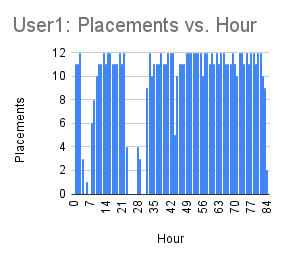
\includegraphics[width=1\linewidth]{visuals/User1_ Placements vs. Hour}
        \end{minipage}
    }
    \subfloat{
        \begin{minipage}{0.315\textwidth}  % Adjust width as needed
            \centering
            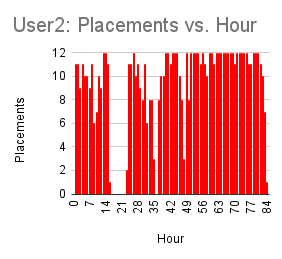
\includegraphics[width=1\linewidth]{visuals/User2_ Placements vs. Hour}
        \end{minipage}
    }
    \subfloat{
        \begin{minipage}{0.315\textwidth}  % Adjust width as needed
            \centering
            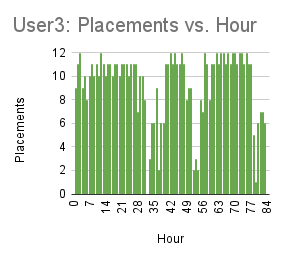
\includegraphics[width=1\linewidth]{visuals/User3_ Placements vs. Hour}
        \end{minipage}
    }
    \caption{User Placements By Hour Since Start}
\end{figure}

\subsection{Why so much activity?}
Given the high probability that these users were not bots or moderators, I assumed that these users must be extremely active members of their communities. With this in mind, the user activity should be focused on specific artwork or community to protect them. Surprisingly, the activity of user 1 and user 2 was somewhat distributed, but user 3 activity was almost solely focused onto one area of the canvas. I plotted the users activity onto the artwork in the area.

\subsubsection{User 3: University of Michigan}

\begin{figure}[H]
    \centering
    \subfloat[\centering UofM Logo]{
        \begin{minipage}{0.15\textwidth}  % Adjust width as needed
            \centering
            
\includegraphics[width=1\linewidth]{visuals/uom}
        \end{minipage}
    }
    \quad
    \subfloat[\centering User 3 Pixels]{
        \begin{minipage}{0.15\textwidth}  % Adjust width as needed
            \centering
            
\includegraphics[width=1\linewidth]{visuals/[280238]_focus_392_252_433_298_259200.0}
        \end{minipage}
    }
    \caption{User 3 Pixels In UofM Logo}
\end{figure}

User 3's pixels are almost all placed in the region of the UofM logo. Additionally user 3's active period, slightly maps to the the day and night cycle when in the EDT time zone, which the state of Michigan uses. 

\subsubsection{User 1 And 2: My Little Pony}

\begin{figure}[H]
    \centering
    \subfloat[\centering Rainbow Dash]{
        \begin{minipage}{0.25\textwidth}  % Adjust width as needed
            \centering
            
\includegraphics[width=1\linewidth]{visuals/rainbowdash}
            
\includegraphics[width=1\linewidth]{visuals/[122804, 78352]_focus_892_1830_961_1885_259200.0.png}
        \end{minipage}
    }
    \quad
    \subfloat[\centering Main Ponies]{
        \begin{minipage}{0.25\textwidth}  % Adjust width as needed
            \centering
            
\includegraphics[width=1\linewidth]{visuals/mlp_6}
            
\includegraphics[width=1\linewidth]{visuals/[122804, 78352]_focus_1614_212_1688_280_259200.0.png}
        \end{minipage}
    }
    \caption{User 1 And 2 Pixels In MLP Art}
\end{figure}

Both User 1 and User 2 had overlapped areas of focus. From this, I conclude that both users are members of the MLP community. This also explains the wider distribution of both users as the MLP community moved their artwork multiple times and had more art that divded their attention. 